\chapter{Preliminaries}

\section{Ergodic Information Theory}
Information theory answers two fundamental questions in communication
theory: What is the ultimate data compression (answer: the entropy $H$),
and what is the ultimate transmission rate of communication (answer: the
channel capacity\footnote{Outside of the scope of this course} $C$ ). For this reason some consider information theory
to be a subset of communication theory. It can be argued that it is much more.
Indeed, it has fundamental contributions to make in statistical physics
(thermodynamics), computer science (Kolmogorov complexity or algorithmic complexity), statistical inference (Occam’s Razor: “The simplest
explanation is best”), and to probability and statistics (error exponents for
optimal hypothesis testing and estimation).
\\Information
theory intersects physics (statistical mechanics), mathematics (probability
theory), electrical engineering (communication theory), and computer science (algorithmic complexity). 

What about ergodicity? The world \textit{ergodic} was introduced by L. Boltzmann in the context of classical (statistical) mechanics to describe the action of the dynamics $T_t, \, t \in \rb$ over an energy surface $\Sigma_E$. Boltzmann had hoped that each orbit $\big\{ T_t, \, t \in \rb \big\}$ would equal the whole energy surface $\Sigma_E$ : he called this statement the \textit{ergodic hypothesis}. The word ergodic comes from the union of the greek words ergon (work) and odos (path). Boltzmann had in fact assumed this hypothesis in order to deduce the equality of time mean and space mean over the phase space, which is a fundamental algorithm in statistical mechanics. 
\\\textit{The ergodic hypothesis, as stated above, is \textbf{false}.} The property that phase flows need to satisfy in order for time and space means of real-valued function is now called \textit{ergodicity}.
\\Usually the term ergodic theory is used to refer to the study of the actions of groups on measure spaces. The actions on topological spaces and smooth manifolds are often called instead topological dynamics and differentiable dynamics. 
\\In the following, we shall study the actions of the group $\mathbb{Z}$ or $\nb$ of integers on a space $\Omega$, i.e. we study a transformation $T: \Omega \longrightarrow \Omega$ (the dynamics of our system) and its iterates $T^n$, $n \in \mathbb{Z}$. 

The main sources for these notes will be Walters \textit{An Introduction to Ergodic Theory} \cite{Walters}, Cover and Thomas \textit{Elements of Information Theory, second edition} \cite{Cover_and_Thomas} and course notes at \url{https://virtuale.unibo.it/course/view.php?id=35914}.

\section{Measure spaces}
\label{par:measure_spaces}
Let $\Omega$ be a set. A $\sigma-$algebra of subsets of $\Omega$ is a collection $\mathscr{B}$ of subsets of $\Omega$ satisfying the following three conditions:
\begin{itemize}
    \item[$1)$] $\Omega \in \mathscr{B}$
    \item[$2)$] if $B \in \mathscr{B}$ then $\Omega \setminus B \in \mathscr{B}$
    \item[$3)$] if $B_n \in \mathscr{B}$ for $n \geq 1$ then $\cup_{n=1}^{\infty} B_n \in \mathscr{B}$.
\end{itemize}
We then call the pair $(\Omega, \mathscr{B})$ a \textit{measurable space}.
\\A \textit{finite measure} on $(\Omega, \mathscr{B})$ is a function $\mu: \mathscr{B} \longrightarrow \rb^+$ satisfying 
\begin{itemize}
    \item[$a:$] $\mu(\emptyset) = 0$
    \item[$b:$] if $B_n \in \mathscr{B}$ are disjoint subsets of $\Omega$ then $\mu \big(\cup_{n=1}^{\infty} B_n\big) = \sum_{n=1}^{\infty} \mu(B_n)$
\end{itemize}
A finite-measure space is a triple $(\Omega, \mathscr{B}, \mu)$ where $(\Omega, \mathscr{B})$ is a measurable space and $\mu$ is a finite measure on $(\Omega, \mathscr{B})$. We say that $(\Omega, \mathscr{B}, \mu)$ is a \textit{probability space}, or normalised measure pace, if $\mu(\Omega) = 1$. We then say that $\mu$ is a probability measure on $(\Omega, \mathscr{B})$. In the following we will usually consider probability spaces. 
\\Another definition that could be useful is that of an algebra:
a collection $\mathscr{A}$ of subsets of $\Omega$ is called an algebra if it satisfies the following three conditions: $i)$ $\emptyset \in \mathscr{A}$ ; $ii)$ if $A, B \in \mathscr{A}$, then $A \cap B \in \mathscr{A}$; $iii)$ if $A \in \mathscr{A}$, then $\Omega \setminus A \in \mathscr{A}$. 
\\Also another mathematical object which is similar to an algebra exists, namely the semi-algebra $\mathscr{C}$. The only difference between $\mathscr{C}$ and $\mathscr{A}$ is that condition $iii)$ of the definition of algebras should be replaced with the looser condition $*)$ if $A \in \mathscr{C}$, then $\Omega \setminus A = \cup_{i=1}^{n} E_i$ where each $E_1 \in \mathscr{C}$ and $E_n, \dots, E_n$ are pairwise disjoint subsets of $\Omega$. From a semi-algebra we can generate an algebra, as stated by the following theorem:
\begin{theorem}
    Let $\mathscr{C}$ be a semi-algebra of subsets of $\Omega$. The algebra $\mathscr{A}(\mathscr{C})$ generated by $\mathscr{C}$ consists precisely of those subsets of $\Omega$ that can be written in the form $E= \cup_{i=1}^{n} A_i$ where each $A_i \in \mathscr{C}$ and $A_1, \dots, A_n$ are disjoint subsets of $\Omega$.
\end{theorem}
We can now define an object which we'll use widely in the following discussions, which is the so called \textit{canonical cilinder}. First, let's define the \textit{measurable rectangles}. For $i \in \zb$ let $(X_i, \mathscr{B}_i, \mu_i)$ be a probability space. Let $X = \prod_{i = -\infty}^{\infty} X_i$. So a point of $X$ is a bisequence $\{x_i\}_{-\infty}^{\infty}$ with $x_i \in X_i$ for each $i$. We now define a $\sigma-$algebra $\mathscr{B}$ of subsets of $X$ called the product of the $\sigma-$algebras $\mathscr{B}_i$. Let $n \geq 0$, let $A_j \in \mathscr{B}_i$ for $|j| \leq n$, and consider the set 

\begin{equation} 
\label{eq:product_space}
    \prod_{i=-\infty}^{-(n+1)} X_i \times \prod_{i=-n}^{n} A_j \times \prod_{i=n+1}^{\infty} X_i = \big\{ (x_i)_{-\infty}^{\infty} \in X \big| x_j \in A_j \, \text{for} \, |j| \leq n \big\} \, .
\end{equation}
Such a set is called a \textit{measurable rectangle} and the collection of all such subsets of $X$ forms a semi-algebra $\mathscr{C}$. It simply represents an infinite bi-sequence for which the symbols from the index $-n$ to $n$ are fixed to be part of the set $A_j$. The $\sigma-$algebra $\mathscr{B}$ is the one generated by $\mathscr{C}$. The measure $\mu_i$ can be extended to $X$ by giving the above rectangle the value $\prod_{j=-n}^{n} \mu_j(A_j)$. The probability space $(X, \mathscr{B}, \mu)$ is called the direct product of the spaces $(X_i, \mathscr{B}_i, \mu_i)$. 
\\A special type of product space will be important for us: the case where each space $(X_i, \mathscr{B}_i, \mu_i)$ is the same space $(\alp, \mathscr{C}, \mu)$ and $\alp$ is a finite set of symbols indexed by an integer $k$, $\{ 0, 1, \dots, k-1 \}$, $\mathscr{C} = 2^{\alp}$, and $\mu$ is given by a probability vector $(p_0,p_1, \dots, p_{k-1})$ where $p_i = \mu(\{i\})$. We call these $\mu(\{i\})$ the \textit{\textbf{marginals}} of $\mu$ and indicate them equivalently as  $\mu(\{k\}) \equiv \mu_k$. We can then take elementary rectangles where each $A_j$ in the description above is taken to be one point of $\alp$. So if $n \geq 0$ and $a_j \in \alp$, $|j| \leq n$, such an elementary rectangle has the form $\{ (x_i)_{-\infty}^{\infty} \big| x_j = a_j \, \text{for} \, |j| \leq n\}$. We shall denote this set by $[x_{-n}^n]$ and call it a \textit{\textbf{canonical cylinder}} or a \textit{block} with end points $-n$ and $n$. 

Let's give a clearer interpretation to all this mathematical description: our space $\alp$ is our \textit{\textbf{alphabet}}, the set which contains all of the symbols we can use: for example this could be, for DNA, the set $\alp= \{ A,C,T,G \}$, or for language the set $\alp = \{ \text{letters of the italian language} \}$. Then we take its product infinite times, as stated in eq. (\ref{eq:product_space}), to be able to consider infinite sequences (for example infinite strings of DNA). We sometimes denote this infinite product as $\Omega \equiv \alp^{\zb}$, to remind ourselves that it is just an infinite product of the same alphabet. Then, we go on to consider infinite sequences for which some characters are fixed: these are our canonical cylinders or blocks. They are nothing more than (infinite) sequences where a certain string of symbols is given. 
\\To make the discussion simpler, most of the times we'll consider just sequences over bisenqueces, and thus consider $\Omega=\alp^{\nb}$. Also we'll mostly use blocks where just the first $n$ symbols are fixed, therefore considering $[x_1^n]$. Of course this is just to make things easier, as everything that will be said in this setting can be then extended to the more general case. 
\\There are some very useful results we could now state, one above all the Kolmogorov Consistency Theorem. But first, let's make a digression about some other preliminaries which will be useful in understanding better all of this Theory of Information.

\section{Topology}
Consider now $\Omega = \alp^{\nb}$. \footnote{Note that the cardinality of $\alp$ grows exponentially, since $|\alp^n| = |\alp|^n$.} It has an elementary topology, induced by a metric. We can define the distance between two characters $z, z' \in \alp$ as 
\begin{equation}
    d_{\alp}(z,z') = 
    \begin{cases}
        1 \quad \text{if} \, z = z' \\
        0 \quad \text{if} \, z \neq z'
    \end{cases}
\end{equation}
Then, given $x,y \in \Omega$ we define the metric
\begin{equation}
    \Tilde{d}(x,y) = \sum_{n=1}^{\infty} 2^{-n} d_{\alp}(x_n, y_n)  
\end{equation}
This function satisfies all properties of a metric. Note that the more two sequences coincide, the smaller $\Tilde{d}$ gets. \\Sometimes it's useful to define another metric: let $\lambda = \frac{1}{|\alp|}$. Define then, given $x,y \in \Omega$,
\begin{equation}
    d_1(x,y) = \lambda^{n(x,y)}
\end{equation}
where $n(x,y) = \min_k \{ k \big| x_k \neq y_k \}$ is the number of the first $n$ different digits of the two sequences. Notice that again, the more prefixes\footnote{the first $m$ digits for a certain $m \in \nb$} coincide, the smaller $d_1$ gets. 
\\The elementary topology in $\Omega$ is generated by defining open sets (or \textit{balls}) in $\Omega$ by means of our distance $d_1$:
\begin{equation*}
    B(x,r) = \big\{ y \in \Omega \big| d_1(x,y) \leq r \big\}
\end{equation*}
These are exactly the $y$'s in our space such that the first $k$ digits coincide up to $\log(r) / \log(\lambda)$, since they satisfy $\lambda^n \leq r$. Thus
\begin{equation}
\label{eq:balls}
    B(x,r) = \big\{ y \in \Omega \big| x_k = y_k \, \text{for} \, 1 \leq k \leq \frac{\log(r)}{\log(\lambda)}\big\}
\end{equation}
We can now identify cylinders and open balls: notice in fact that, from its definition, a cylinder 
\begin{equation*}
    [x_1^n] = \bigg\{ y \big| \, 
    \begin{matrix}
        y_1 = x_1 \\
        \vdots \\
        y_n = x_n
    \end{matrix}
    \bigg\}    
\end{equation*}
coincides with the open sets defined in eq. (\ref{eq:balls}) 
\begin{equation}
    [x_1^{ \frac{\log(r)}{\log(\lambda)}}] = B(x,r) 
\end{equation}
Therefore the canonical cylindera are generators of our topology in $\Omega$. 
\\Also, it can be proven that the two distances $\Tilde{d}$ and $d_1$ induce the same topology, i.e. that open balls defined by $\Tilde{d}$ are contained in open balls defined by $d_1$, and viceversa.

\section{Lebesgue Integration}

\cite{Wikipedia} The integral of a positive function $f$ between limits $a$ and $b$ can be interpreted as the area under the graph of f. This is straightforward for functions such as polynomials, but what does it mean for more exotic functions? In general, for which class of functions does "area under the curve" make sense? The answer to this question has great theoretical and practical importance. \\
As part of a general movement toward rigor in mathematics in the nineteenth century, mathematicians attempted to put integral calculus on a firm foundation. The Riemann integral—proposed by Bernhard Riemann (1826–1866)—is a broadly successful attempt to provide such a foundation. Riemann's definition starts with the construction of a sequence of easily calculated areas that converge to the integral of a given function. This definition is successful in the sense that it gives the expected answer for many already-solved problems, and gives useful results for many other problems.\\
However, Riemann integration does not interact well with taking limits of sequences of functions, making such limiting processes difficult to analyze. This is important, for instance, in the study of Fourier series, Fourier transforms, and other topics. The Lebesgue integral is better able to describe how and when it is possible to take limits under the integral sign (via the monotone convergence theorem and dominated convergence theorem).\\
While the Riemann integral considers the area under a curve as made out of vertical rectangles, the Lebesgue definition considers horizontal slabs that are not necessarily just rectangles, and so it is more flexible. For this reason, the Lebesgue definition makes it possible to calculate integrals for a broader class of functions. For example, the Dirichlet function, which is $0$ where its argument is irrational and $1$ otherwise, has a Lebesgue integral, but does not have a Riemann integral. Furthermore, the Lebesgue integral of this function is zero, which agrees with the intuition that when picking a real number uniformly at random from the unit interval, the probability of picking a rational number should be zero.
Folland ($1984$) summarizes the difference between the Riemann and Lebesgue approaches thus: "to compute the Riemann integral of $f$, one partitions the domain $[a, b]$ into subintervals", while in the Lebesgue integral, "one is in effect partitioning the range of $f$." \\
For the Riemann integral, the domain is partitioned into intervals, and bars are constructed to meet the height of the graph. The areas of these bars are added together, and this approximates the integral, in effect by summing areas of the form $f(x)dx$ where $f(x)$ is the height of a rectangle and $dx$ is its width.\\
For the Lebesgue integral, the range is partitioned into intervals, and so the region under the graph is partitioned into horizontal "slabs" (which may not be connected sets). The area of a small horizontal "slab" under the graph of $f$, of height $dy$, is equal to the measure of the slab's width times $dy$: $\mu\big( \{ x \big| f(x) > y \} \big)$.
The Lebesgue integral may then be defined by adding up the areas of these horizontal slabs. See as an example Fig. \ref{fig:leb1}.

\begin{figure}[h]
    \centering
    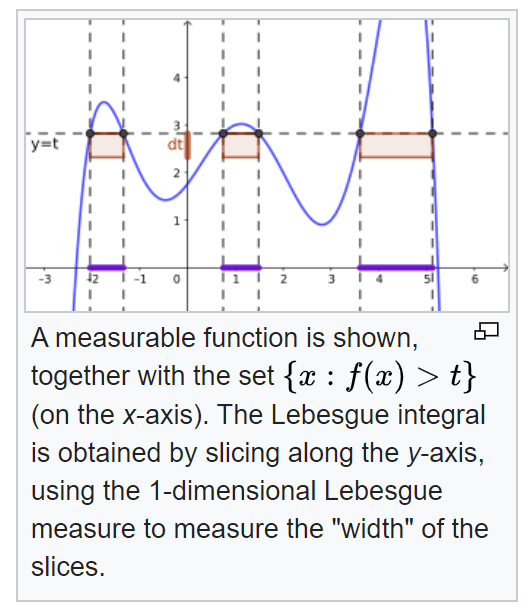
\includegraphics[width=7cm]{img/leb1.png}
    \caption{}
    \label{fig:leb1}
\end{figure}
An equivalent way to introduce the Lebesgue integral is to use so-called simple functions, which generalize the step functions of Riemann integration. Consider, for example, determining the cumulative COVID-19 case count from a graph of smoothed new daily cases (Fig. \ref{fig:leb2}). 
\begin{itemize}
    \item[*]\textbf{The Riemann–Darboux approach}
    \\Partition the domain (time period) into intervals (eight, in the example at right) and construct bars with heights that meet the graph. The cumulative count is found by summing, over all bars, the product of interval width (time in days) and the bar height (cases per day).
    \item[*]\textbf{The Lebesgue approach}
    \\Choose a finite number of target values (eight, in the example) in the range of the function. By constructing bars with heights equal to these values, but below the function, they imply a partitioning of the domain into the same number of subsets (subsets, indicated by color in the example, need not be connected). This is a "simple function," as described below. The cumulative count is found by summing, over all subsets of the domain, the product of the measure on that subset (total time in days) and the bar height (cases per day).
\end{itemize}

\begin{figure}[h]
    \centering
    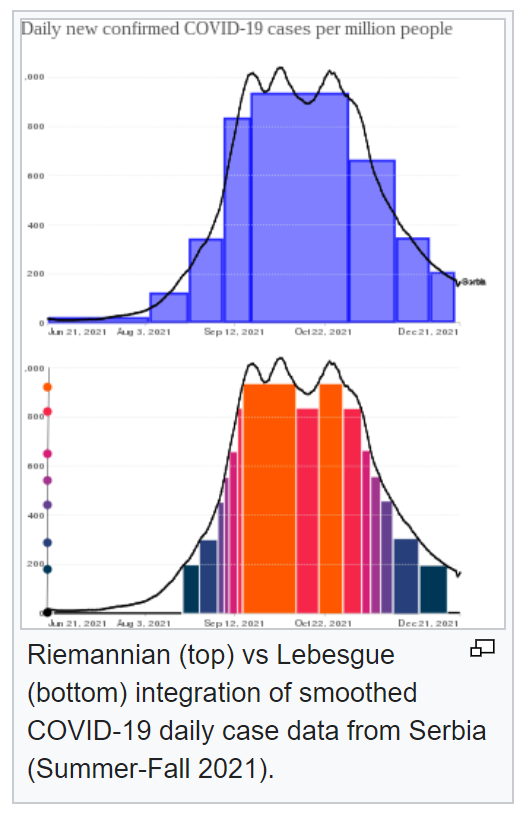
\includegraphics[width=7cm]{img/leb2.png}
    \caption{}
    \label{fig:leb2}
\end{figure}

Let's now go back to the mathematics and give a rigorous formulation of the Lebesgue integral.\\
Let $\mathscr{B}(\rb)$ denote the $\sigma$-algebra of Borel subsets of $\rb$. This is the $\sigma$-algebra generated by all open subsets of $\rb$ and is also generated by the collection of all intervals, or by the collection of all intervals of the form $(c, \infty)$. 
\\Let $(X, \mathscr{B}, m)$ a measure space. A function $f: X \rightarrow \rb$ is \textit{measurable} if $f^{-1}(D) \in \mathscr{B}$ whenever $D \in \mathscr{B}(\rb)$ or equivalently if $f^{-1}(c, \infty) \in \mathscr{B}$ for all $c \in \rb$. A function $f: X \rightarrow \mathbb{C}$ is measurable if both its imaginary and real part are measurable. We say $f=g$ \textit{almost everywhere} (a.e.) if $m\big( 
\{ x: f(x) \neq g(x) \} \big) = 0$, i.e. the functions have equal values everywhere except for a set which has null measure.\footnote{If the only open set of zero measure in a topological space $X$ is the void set, then being equal a.e. for $f$ and $g$ implies being equal. } In measure theory, all sets of null measure are "invisible". 
\\Let $(X, \mathscr{B}, m)$ be a probability space. A function $f: X \rightarrow \rb$ is a \textit{simple function} if it can be written in the form $\sum_{i=1}^n a_i \chi_{A_i}$, where $a_i \in \rb$, $A_i \in \mathscr{B}$, the sets $A_i$ are disjoint sets of $X$, and $\chi_{A_i}$ denotes the characteristic function of $A_i$ ($\chi(x) = 1$ if $x \in A_i$, $0$ otherwise). Simple functions are measurable. We define the integral for simple functions by:
\begin{equation}
    \label{eq:simple_functions_integral}
    \int f \, dm = \sum_{i=1}^n a_i m(A_i) \, .
\end{equation}
This value is independent of the representation $\sum_{i=1} a_i \chi_{A_i}$.  
\\Suppose $f: X \rightarrow \rb$ is measurable and $f \geq 0$. Then there exists an increasing sequence of simple functions $f_n \rightarrow f$. For example, we could take
\begin{equation*}
    f_n(x) = 
    \begin{cases}
        \frac{i-1}{2^n}, \:& \text{if} \, \frac{i-1}{2^n} \leq f(x) \leq \frac{i}{2^n} \: i = 1, \dots, n2^n \\
        n, & \text{if} \, f(x) \geq n \, .
    \end{cases}
\end{equation*}
We define $\int f \, dm = \lim_{n \rightarrow \infty} \int f_n \, dm$ and note that this definition is independent of the chosen sequence $\{ f_n \}$. We say $f$ is \textit{integrable} if $\int f \, dm < \infty$. 
\\Suppose $f:X \rightarrow \rb$ is measurable. Then $f = f^+ - f^-$ where $f^+(x) = \max \{f(x), 0 \} \geq 0$ and $f^- = \max \{ -f(x), 0 \} \geq 0$. We say that $f$ is integrable if $\int f^+ dm$, $\int f^- dm < \infty$ and we then define 
\begin{equation*}
    \int f \, dm = \int f^+ dm - \int f^- dm
\end{equation*}
Notice that $f$ is (Lebesgue-)integrable if and only if $|f|$ is integrable. If $f=g$ a.e. then one is integrable if the other is and $\int f \, dm = \int g \, dm$. 
\\The main theorems on integrating sequences as functions are the following: 
\begin{theorem}[Dominated Convergence Theorem]
Suppose $f_1 \leq f_2 \leq f_3 \leq \dots$ is an increasing sequence of integrable real-valued functions on $(X, \mathscr{B}, m)$. If $\big\{ \int f_n \, dm \big\}$ is a bounded sequence of real numbers, then $\lim_{n \rightarrow \infty} f_n$ exists a.e. and is integrable and $\int (\lim_{n \rightarrow \infty} f_n) dm = \lim_{n \rightarrow \infty} \int f_n$. If instead $\big\{ \int f_n \, dm \big\}$ is an unbounded sequence then either $\lim_{n \rightarrow \infty} f_n$ is infinite on a set of not zero measure or $\lim_{n \rightarrow \infty} f_n$ is not integrable. 
\end{theorem}
\begin{lemma}[Fatou's Lemma]
Let $\{ f_n \}$ be a sequence of measurable real-valued functions on $(X, \mathscr{B}, m)$ which is bounded below by an integrable function. If $\liminf_{n\rightarrow\infty} \int f_n \, dm < \infty$ then $\liminf_{n\rightarrow\infty} f_n$ is integrable and $\int 
 \liminf_{n\rightarrow\infty} f_n \, dm \leq \liminf_{n\rightarrow\infty} \int f_n \, dm$
 \end{lemma}
 
\begin{corollary}[Dominated Convergence Theorem]
 If $g:X \rightarrow \rb$ is integrable and $\{ f_n \}$ is a sequence of measurable real-valued functions with $|f_n| \leq g$ a.e. and $\lim_{n\rightarrow\infty} f_n = f$ a.e. then f is integrable and $\lim_{n\rightarrow\infty} \int f_n \, dm = \int f \, dm$. 
 \end{corollary}
We denote by $L^1(X)$ the space of all Lebesgue integrable functions. Such space is a Banach space with norm $\|f\|_1 = \int |f| \, dm$. If $f \in L^1(X)$, then $\int_A f \, dm$ denotes $\int f \cdot \chi_A \, dm$. 

\section{Perron-Frobenius Theory}
\label{par:perron_frobenius_theory}
In matrix theory, the Perron–Frobenius theorem, proved by Oskar Perron $(1907)$ and Georg Frobenius $(1912)$, asserts that a real square matrix with positive entries has a unique largest real eigenvalue and that the corresponding eigenvector can be chosen to have strictly positive components, and also asserts a similar statement for certain classes of non-negative matrices.
\\This theorem has important applications to probability theory (ergodicity of Markov chains); to the theory of dynamical systems (subshifts of finite type); to economics (Okishio's theorem, Hawkins–Simon condition); to demography (Leslie population age distribution model); to social networks (DeGroot learning process); to Internet search engines (PageRank); and even to ranking of football teams.
\\Let $A=[a_{ij}]$ be a $k \times k$ matrix. We say $A$ is non-negative if $a_{ij} \geq 0$ for all $i,j$. Such a matrix is called \textit{irreducible} if for any pair $i,j$ there is some $n>0$ such that $a_{ij}^{(n)}>0$ where $a_{ij}^{(n)}$ is the $(i,j)$-th element of $A^n$. The matrix $A$ is \textit{irreducible} and \textit{aperodic} if there exists $n>0$ such that $a_{ij}^{(n)} >0$ for \textit{all} $i,j$. We shall use the following result:
\begin{theorem}[Perron-Frobenius Theorem]
    Let $A = [a_{ij}]$ be a non-negative $k \times k$ matrix. Then:
    \begin{itemize}
        \item[(i)] There is a non negative eigenvalue $\lambda$ such that no eigenvalue of $A$ has absolute value greater than $\lambda$.
        \item[(ii)] We have $\min_i( \sum_{j=1}^k a_{ij}) \leq \lambda \leq \max_i( \sum_{j=1}^k a_{ij})$
        \item[(iii)] Corresponding to the eigenvalue $\lambda$ there is a non-negative left (row) eigenvector $u = (u_1, \dots, u_k)$ and a non-negative right (column) eigenvector
        \begin{equation*}
        v = 
            \begin{pmatrix}
                v_1 \\
                \vdots \\
                v_k
            \end{pmatrix}
        \end{equation*}
        \item[(iv)] If $A$ is irreducible then $\lambda$ is a simple eigenvalue and the corresponding eigenvectors are strictly positive (i.e. $u_i >0$, $v_i >0$ $\forall i$).
        \item[(v)] If $A$ is irreducible then $\lambda$ is the only eigenvalue of $A$ with a non-negative eigenvector.
    \end{itemize}
\end{theorem}
This result, as already said, will become very useful when we'll talk about Markov Chain and Hidden Markov Models.

